\documentclass[11pt,a4paper]{article}
\usepackage[margin=2.4cm]{geometry}
\usepackage{amsmath,amssymb}
\usepackage{graphicx}
\usepackage{booktabs}
\usepackage{caption}
\usepackage{xcolor}
\usepackage[hidelinks]{hyperref}
\usepackage[expansion=false]{microtype}
\usepackage{enumitem}

\captionsetup{font=small,labelfont=bf}
\setlist{itemsep=2pt,topsep=4pt}
\newcommand{\E}{\mathbb{E}}
\newcommand{\Q}{\mathbb{Q}}
\renewcommand{\P}{\mathbb{P}}

\title{\textbf{quantdesk: Building and Testing an\\Options Research Desk from First Principles}}
\author{Mohammed Alazemi\\[2pt]\small BSc Physics, The University of Manchester\\
\small\href{https://github.com/Mohammed-Alazemi/quantdesk}{\texttt{github.com/Mohammed-Alazemi/quantdesk}}}
\date{\small October 2026}

\begin{document}
\maketitle

\begin{abstract}
\noindent
This paper describes \texttt{quantdesk}, a Python library I wrote to turn an options trade idea into a decision: what it is worth, what it is exposed to, how much to risk, and whether the evidence for it is real. It covers:
\begin{itemize}[leftmargin=1.5em]
  \item Black--Scholes pricing and the Greeks;
  \item volatility forecasting with GARCH and smile fitting with SVI;
  \item semi-analytic Heston pricing and calibration;
  \item a delta-hedging simulator;
  \item risk-neutral densities, variance swaps and earnings event volatility;
  \item Kelly sizing;
  \item backtest statistics that correct for luck and for trying many ideas;
  \item an inventory-aware market maker.
\end{itemize}
The rule throughout was the one I learned in physics: \emph{a model is not trusted until it reproduces a result whose answer is known}. Each of the 43 automated tests checks the code against a closed-form result, an independent numerical method, or a published table. I explain the mathematics behind each part, how I built and checked it, and what it taught me. The most useful lesson was that the code works, but the earnings strategy I trade does not yet have a proven edge.
\end{abstract}

\section{Why I built it}
I trade listed options on US large caps to a written rulebook. My first tool was a single script: Black--Scholes prices, a GARCH volatility forecast, a Monte Carlo of the trade, Kelly sizing and a seven-gate checklist. It gave confident answers, but nothing in it showed whether those answers were right. This project rebuilt that script as a tested library and extended it until each question a trader should ask had a tool behind it:
\begin{itemize}[leftmargin=1.5em]
  \item What is this option worth?
  \item What does the market's smile imply?
  \item Where does the P\&L actually come from?
  \item How much should I risk?
  \item Is my backtest lying to me?
\end{itemize}

\section{Pricing: Black--Scholes, the Greeks and implied volatility}
\paragraph{Model.} The stock follows geometric Brownian motion, $dS = \mu S\,dt + \sigma S\,dW$. Itô's lemma applied to an option value $V(S,t)$ gives
\begin{equation}
dV = \Big(\partial_t V + \mu S\,\partial_S V + \tfrac12\sigma^2S^2\partial_{SS}V\Big)dt + \sigma S\,\partial_S V\,dW .
\end{equation}
Hold the option and short $\Delta=\partial_S V$ shares. The $dW$ terms cancel, so the portfolio is riskless and must earn the risk-free rate $r$. That gives the Black--Scholes equation
\begin{equation}
\partial_t V + \tfrac12\sigma^2S^2\partial_{SS}V + (r-q)S\,\partial_S V - rV = 0 .
\end{equation}
The drift $\mu$ has disappeared: an option prices volatility, not direction. For a call with dividend yield $q$,
\begin{equation}
C = Se^{-qT}N(d_1) - Ke^{-rT}N(d_2),\qquad d_{1,2} = \frac{\ln(S/K) + (r-q\pm\frac12\sigma^2)T}{\sigma\sqrt T}.
\end{equation}

\paragraph{What I built.}
\begin{itemize}[leftmargin=1.5em]
  \item \textbf{Prices and Greeks.} Vectorised prices and seven Greeks: $\Delta$, $\Gamma$, vega, $\Theta$, $\rho$, vanna and volga.
  \item \textbf{Implied volatility.} A solver that first checks the no-arbitrage bounds
  \[\max(Se^{-qT}-Ke^{-rT},\,0) < C < Se^{-qT},\]
  then finds the root with Brent's method. It returns NaN instead of a meaningless number when a quote violates the bounds.
  \item \textbf{American options.} A Cox--Ross--Rubinstein binomial tree with early exercise.
\end{itemize}

\paragraph{How I checked it.} Table~\ref{tab:valid} lists every check in the library. The pricing checks are:
\begin{itemize}[leftmargin=1.5em]
  \item put--call parity holds to $10^{-14}$;
  \item the textbook price $C(100,100,1,5\%,20\%) = 10.4506$ is reproduced;
  \item implied vol round-trips to machine precision;
  \item every Greek matches a central finite difference to $10^{-6}$.
\end{itemize}
The American put is worth $10.377$, against $10.109$ for the European, so the early-exercise premium is positive, as it must be. The American call with no dividends equals the European call, as theory requires.

\section{Volatility: GARCH forecasts and the SVI smile}
\paragraph{GARCH(1,1).} Daily variance follows $h_t = \omega + \alpha r_{t-1}^2 + \beta h_{t-1}$. I fit it by maximum likelihood, $\min \frac12\sum(\ln h_t + r_t^2/h_t)$, with \emph{variance targeting}: I fix $\omega = V(1-\alpha-\beta)$ at the sample variance $V$ and fit only $(\alpha,\beta)$. A free three-parameter fit on a few hundred returns often wandered to absurd values; the two-parameter fit is stable.

The forecast of average variance over a horizon of $H$ days uses the mean reversion $h_{t+k} = V + (\alpha+\beta)^k(h_{t+1} - V)$. This forecast, not last month's realised vol, is what an option's implied vol should be compared against. To check the fit, I simulated a GARCH process with known parameters: the fit recovers $\alpha$ to within $0.02$ and $\beta$ to within $0.03$.

\paragraph{SVI.} Gatheral's raw SVI parametrises total implied variance $w = \sigma_{\rm imp}^2T$ in log-moneyness $k=\ln(K/F)$:
\begin{equation}
w(k) = a + b\big(\rho(k-m) + \sqrt{(k-m)^2+s^2}\big).
\end{equation}
A fitted smile can still contain \emph{butterfly arbitrage}, meaning a negative probability density. I implemented Gatheral's condition $g(k)\ge 0$, which flags such smiles.

\section{Stochastic volatility: semi-analytic Heston}
Black--Scholes assumes constant volatility, but real smiles are skewed: downside strikes trade at higher implied vol. Heston's model lets variance $v$ follow its own mean-reverting process, correlated with the stock:
\begin{equation}
dS = (r-q)S\,dt + \sqrt v\,S\,dW_1,\qquad dv = \kappa(\theta - v)\,dt + \xi\sqrt v\,dW_2,\qquad dW_1dW_2 = \rho\,dt .
\end{equation}

\paragraph{Pricing.} The characteristic function $\varphi(u) = \E^\Q[e^{iuX}]$ of $X=\ln(S_T/F)$ is known in closed form. I used the ``little trap'' version of Albrecher et al., which avoids a branch-cut discontinuity in Heston's original expression at long maturities:
\begin{align}
\varphi(u) &= \exp\!\Big\{\tfrac{\kappa\theta}{\xi^2}\Big[(a-d)T - 2\ln\tfrac{1-ge^{-dT}}{1-g}\Big] + \tfrac{v_0}{\xi^2}(a-d)\tfrac{1-e^{-dT}}{1-ge^{-dT}}\Big\},\\
a &= \kappa - \rho\xi iu,\quad d = \sqrt{a^2 + \xi^2(iu+u^2)},\quad g = \tfrac{a-d}{a+d}. \nonumber
\end{align}
Prices then follow from Lewis's single integral,
\begin{equation}
C = Se^{-qT} - \frac{\sqrt{FK}\,e^{-rT}}{\pi}\int_0^\infty \frac{\mathrm{Re}\big[e^{iu\ln(F/K)}\varphi(u - \tfrac i2)\big]}{u^2+\tfrac14}\,du .
\end{equation}
I evaluate the integral on 256 fixed Gauss--Legendre nodes after the substitution $u = c\,t/(1-t)$. The scale $c$ is set by the total variance, so the nodes sit where the integrand lives for both short and long maturities. Fixed nodes make the price a smooth function of the parameters, which matters for calibration. Pricing 30 strikes takes about 0.3\,ms.

\paragraph{Calibration.} I fit $(v_0,\kappa,\theta,\xi,\rho)$ by least squares on price errors divided by Black--Scholes vega. To first order this is an implied-vol error, but it avoids inverting every model price inside the optimiser. The fit runs from several starting points to avoid local minima.

\paragraph{How I checked it.} I tested the pricer four ways:
\begin{itemize}[leftmargin=1.5em]
  \item it equals Black--Scholes to $10^{-6}$ in the limit $\xi\to0$, $\rho=0$;
  \item it matches adaptive quadrature to $10^{-8}$;
  \item it agrees with my independent Monte Carlo simulator within its standard error;
  \item it satisfies put--call parity.
\end{itemize}
Calibrating to a surface the model generated itself recovers all five parameters to a relative error of $10^{-4}$. Figure~\ref{fig:heston} shows the harder test: 45 quotes over five expiries with $0.2$ vol points of noise added.

\begin{figure}[t]
\centering
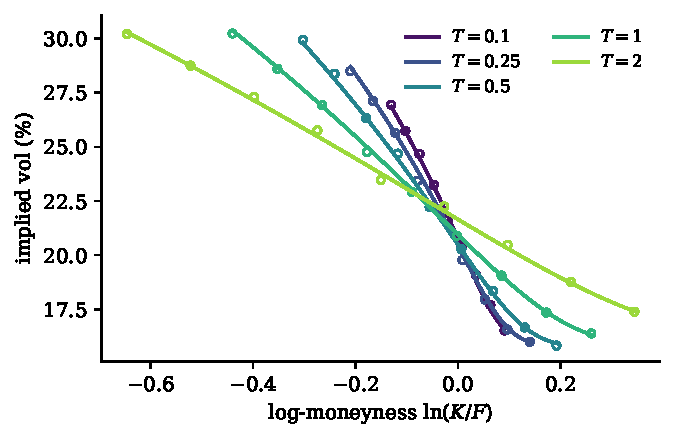
\includegraphics[width=0.6\linewidth]{figures/fig1_heston.pdf}
\caption{Heston calibrated to 45 noisy implied-vol quotes (circles) across five expiries (lines are the fitted model). The fitted parameters $(v_0,\kappa,\theta,\xi,\rho) = (0.045, 2.55, 0.060, 0.69, -0.71)$ compare with the true $(0.045, 2.50, 0.060, 0.70, -0.70)$. The residual is 0.16 vol points, just below the 0.2-point noise level, which is what a correct fit should give.}
\label{fig:heston}
\end{figure}

\section{Where an option trader's P\&L comes from}
This section was the most valuable to me, because it explains my own trades. Buy an option at implied vol $\sigma_i$ and delta-hedge it while the stock moves with realised vol $\sigma_r$. Over $dt$, the hedged position (option minus $\Delta_i$ shares, financed at $r$) gains
\begin{equation}
d\Pi = \tfrac12\Gamma_i S^2\big(\sigma_r^2 - \sigma_i^2\big)\,dt ,
\end{equation}
because the option's theta exactly pays for gamma at the implied vol. So the hedged P\&L is a bet on realised against implied volatility. There are two hedging choices (Wilmott, ch.~10):
\begin{itemize}[leftmargin=1.5em]
  \item \textbf{Hedge at $\sigma_r$.} The P\&L is deterministic in the continuous limit: $[V(\sigma_r) - V(\sigma_i)]\,e^{rT}$. The edge is locked in.
  \item \textbf{Hedge at $\sigma_i$.} The expected P\&L has the same sign, but it is $\int e^{r(T-t)}\frac12\Gamma_iS^2(\sigma_r^2-\sigma_i^2)dt$. That depends on the path, because $\Gamma$ is large only while the stock stays near the strike.
\end{itemize}
Real hedging is discrete. With $n$ rebalances and no vol edge, each step leaves an error proportional to $\Gamma S^2\sigma^2(Z^2-1)\Delta t$. Kamal and Derman showed that the total has standard deviation $\approx \sqrt{\pi/4}\;\nu\,\sigma/\sqrt n$ for an at-the-money option, where $\nu$ is vega.

\paragraph{What I built and found.} I wrote a vectorised hedging simulator (20{,}000 antithetic paths, optional transaction costs). In it, a 6-month ATM call is bought at $\sigma_i=20\%$ while the stock realises $\sigma_r=30\%$. Figure~\ref{fig:hedge} shows four results:
\begin{itemize}[leftmargin=1.5em]
  \item \textbf{Hedging at $\sigma_r$ converges to the locked-in \$2.82.} The spread halves each time the number of rebalances is multiplied by four.
  \item \textbf{Hedging at $\sigma_i$ has the same mean, but its spread levels off near \$1.3} however often you rebalance: that remainder is the path dependence.
  \item \textbf{With no edge, the simulated hedging error matches Derman--Kamal} to within a few percent at every $n$.
  \item \textbf{The hedged P\&L does not depend on the stock's drift:} the means at $\mu = -30\%$, $0\%$ and $+40\%$ agree to within 3 cents.
\end{itemize}

\begin{figure}[t]
\centering
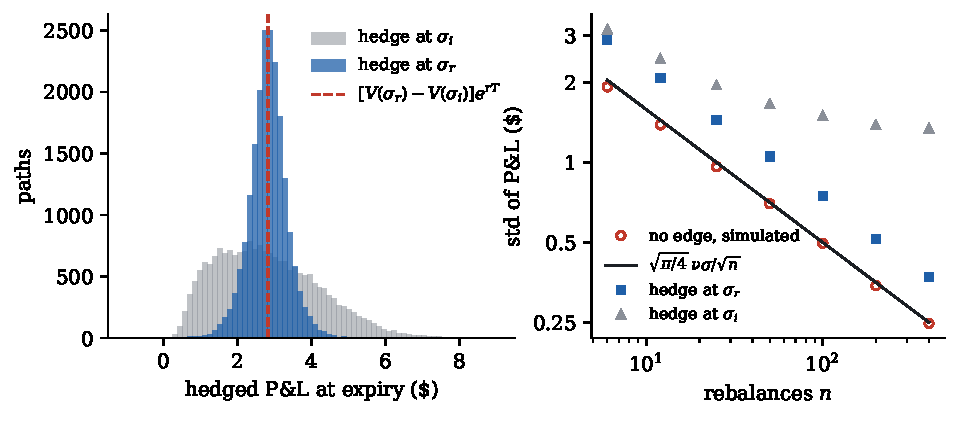
\includegraphics[width=\linewidth]{figures/fig2_hedging.pdf}
\caption{Delta hedging an ATM call bought at 20\% implied vol while the stock realises 30\%. \textbf{Left:} P\&L after 200 rebalances. Hedging at the realised vol concentrates it on the locked-in value (dashed); hedging at the implied vol leaves a wide, path-dependent spread. \textbf{Right:} the standard deviation of P\&L against the number of rebalances. Circles: no vol edge, compared with the Derman--Kamal formula (line).}
\label{fig:hedge}
\end{figure}

\section{What the smile prices in}
\paragraph{Risk-neutral density.} Differentiating $C(K) = e^{-rT}\int (S-K)^+ f(S)\,dS$ twice with respect to the strike gives Breeden and Litzenberger's result
\begin{equation}
f(K) = e^{rT}\,\frac{\partial^2 C}{\partial K^2}.
\end{equation}
The option market therefore prices a full probability distribution, not only a volatility. I take the second difference of prices generated from a smooth SVI smile. With flat volatility, it recovers the lognormal density to $10^{-6}$. For the skewed smile in Fig.~\ref{fig:density}, the density integrates to $1.0000$ and has the forward as its mean, with skewness $-0.68$ and excess kurtosis $3.1$. That is a fat left tail which a single volatility number cannot describe.

\paragraph{Variance swap.} The payoff of a log contract can be replicated with a static strip of options. Since $\int\sigma^2dt = 2\big(\int dS/S - \ln(S_T/S_0)\big)$, the fair strike of a variance swap is
\begin{equation}
K_{\rm var} = \frac{2e^{rT}}{T}\Big[\int_0^F \frac{P(K)}{K^2}dK + \int_F^\infty \frac{C(K)}{K^2}dK\Big].
\end{equation}
Checks: flat vol returns $\sigma^2$ to $10^{-4}$. On the skewed smile the variance-swap volatility is $28.3\%$, against $22.4\%$ at the money. The difference is what the skew costs.

\paragraph{Earnings event volatility.} Variance adds across days. If an expiry $n$ trading days away contains one event day, then $\sigma_{\rm term}^2\,n = \sigma_E^2 + \sigma_{\rm reg}^2(n-1)$. With a term IV of 36\%, a normal-day vol of 24\% and $n=40$, the event day carries $\sigma_E = 171\%$ annualised. That implies an expected absolute move of $\sigma_E\sqrt{2/\pi}/\sqrt{252} = 8.6\%$. Removing $\sigma_E$ after the print predicts the IV crush before it happens. This is the arithmetic behind my rule ``never hold through earnings''.

\begin{figure}[t]
\centering
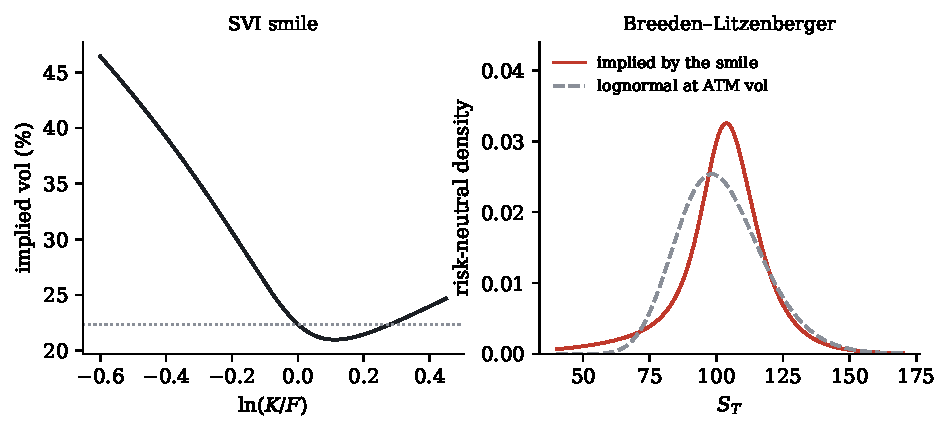
\includegraphics[width=\linewidth]{figures/fig3_density.pdf}
\caption{\textbf{Left:} a skewed SVI smile (dotted line: ATM vol). \textbf{Right:} the risk-neutral density it implies (Breeden--Litzenberger), against a lognormal with the same ATM vol. The skew moves probability into the left tail and makes the centre narrower.}
\label{fig:density}
\end{figure}

\section{From a model to a decision: sizing}
\paragraph{Monte Carlo under the real-world measure.} Prices are expectations under the risk-neutral measure $\Q$, where every asset drifts at $r$. My P\&L, however, happens under the real-world measure $\P$, with drift $\mu$. The library therefore prices the option with market implied vol and simulates the trade under my own drift and volatility forecast. The simulation uses GBM, or Heston with a path-dependent exit IV, and every fill pays half the bid--ask spread plus commission.

\paragraph{Kelly.} For a return on premium $R$, the growth-optimal fraction maximises $g(f) = \E[\ln(1+fR)]$. For a binary bet that wins $b$ with probability $p$, the optimum is $f^* = p - (1-p)/b$. Option returns are skewed and bounded at $-100\%$, so the library maximises $g$ directly over the simulated returns: a grid search refined by a bounded one-dimensional search. On a bet that wins $1.5\times$ or loses $1\times$ at $p=\frac12$, it returns $0.1655$ against the exact $\frac16$; the difference is sampling noise.

Since $g(f)\approx f\mu - \frac12f^2\sigma^2$, half-Kelly keeps 75\% of the growth with half the volatility, and that is the default. A bootstrap of $f^*$ shows how fragile the estimate is. A sweep over assumed drifts shows whether an apparent edge exists only under an optimistic drift. In my demo it did: the Kelly fraction is $0\%$ at every drift up to $20\%$ a year.

\paragraph{The rulebook.} My trading rules are an editable \texttt{Rules} object with eight hard gates:
\begin{enumerate}[leftmargin=1.5em]
  \item probability of profit;
  \item Sharpe per trade;
  \item Kelly fraction above zero;
  \item IV no more than 15\% above HV30;
  \item at least 45 days to expiry;
  \item exit before earnings;
  \item position no larger than 10\% of the portfolio;
  \item a limit on the number of open positions.
\end{enumerate}
Soft gates warn. A size is suggested only if every hard gate passes.

\section{Is the backtest lying?}
\paragraph{The strategy and its result.} My main strategy buys an at-the-money call about six weeks before earnings and sells it the day before the print, to catch the run-up in implied vol. I backtested it on synthetic markets in which I control the size of the pre-earnings IV ``pump''. The backtest uses realistic costs and 20 tickers $\times$ 39 events. Table~\ref{tab:bt} shows the result:
\begin{itemize}[leftmargin=1.5em]
  \item \textbf{With a 35\% pump, the strategy only breaks even.} Theta and costs eat the gain.
  \item \textbf{With no pump, it loses $9.2\%$ per trade}, a loss that is clearly significant.
  \item \textbf{A null test that places the same trade on random dates} shows whether timing adds anything at all.
\end{itemize}

\begin{table}[t]
\centering\small
\begin{tabular}{lcccc}
\toprule
Synthetic market & trades & mean return on premium (95\% CI) & $t$ & $P(\text{Sharpe}>0)$\\
\midrule
No IV pump & 780 & $-9.2\%$ \;($-15.1\%$, $-3.2\%$) & $-3.04$ & 0.3\% \\
35\% IV pump & 780 & $-0.2\%$ \;($-5.8\%$, $+5.2\%$) & $-0.08$ & 47\% \\
\midrule
\multicolumn{5}{l}{Expiry after the print (35\% pump): 14 d $-8.9\%$ \;|\; 45 d $-0.2\%$ \;|\; 90 d $+4.7\%$ \;|\; 120 d $+6.3\%$}\\
\bottomrule
\end{tabular}
\caption{Pre-earnings IV-pump backtest with costs, on synthetic data where the pump is put in by construction.}
\label{tab:bt}
\end{table}

\paragraph{Overfitting.} Longer expiries look better in Table~\ref{tab:bt}, but I found that by trying several. Trying many variants and keeping the best inflates the Sharpe ratio. Two statistics from Bailey and López de Prado correct for this. The \emph{probabilistic Sharpe ratio} is
\begin{equation}
\mathrm{PSR}(SR^*) = N\!\left(\frac{(\widehat{SR} - SR^*)\sqrt{n-1}}{\sqrt{1 - \gamma_3\widehat{SR} + \frac{\gamma_4-1}{4}\widehat{SR}^2}}\right),
\end{equation}
which accounts for sample length, skewness $\gamma_3$ and kurtosis $\gamma_4$. The \emph{deflated} Sharpe ratio sets the benchmark $SR^*$ to the expected maximum Sharpe of $N$ skill-less trials,
\begin{equation}
SR^* = \sigma_{SR}\Big[(1-\gamma)N^{-1}(1-\tfrac1N) + \gamma N^{-1}(1-\tfrac1{Ne})\Big],
\end{equation}
where $\gamma$ is the Euler--Mascheroni constant. Figure~\ref{fig:dsr} shows the test I used. Among 100 random strategies, the best has a median annualised Sharpe of 2.4. The naive test calls it skilled in 99.7\% of trials; the deflated test does so in none of 300 trials. The library also provides walk-forward splits with an embargo, so that parameters are never tuned on the period they are tested on.

\begin{figure}[t]
\centering
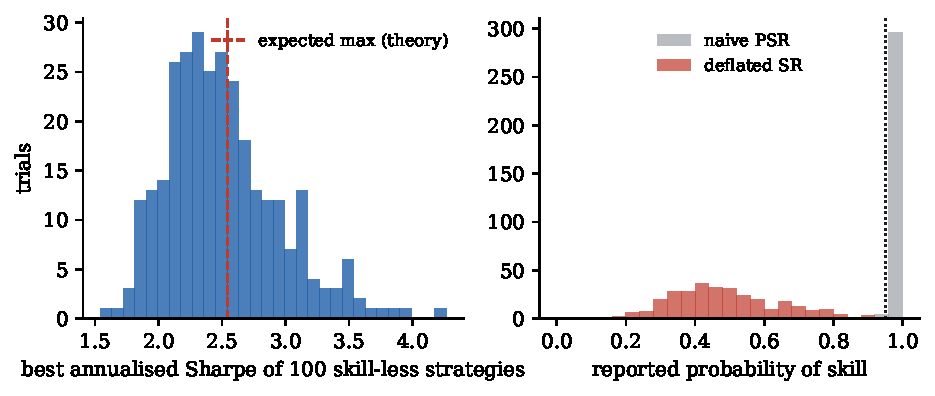
\includegraphics[width=\linewidth]{figures/fig4_overfitting.pdf}
\caption{Selection bias. \textbf{Left:} the best annualised Sharpe among 100 skill-less strategies (250 days each), over 300 trials, with the theoretical expected maximum marked. \textbf{Right:} the probability of skill reported for that best strategy. The naive PSR almost always passes the 95\% line (dotted); the deflated Sharpe ratio never does.}
\label{fig:dsr}
\end{figure}

\section{Market making with inventory risk}
A market maker earns the spread but carries inventory $q$. Avellaneda and Stoikov model fills as arriving at rate $Ae^{-k\delta}$ for a quote $\delta$ away from the mid, and give the market maker exponential utility with risk aversion $\gamma$. The optimal quotes centre on a reservation price that shifts against inventory:
\begin{equation}
r = s - q\gamma\sigma^2(T-t),\qquad \delta_a + \delta_b = \gamma\sigma^2(T-t) + \tfrac{2}{\gamma}\ln\!\big(1 + \tfrac{\gamma}{k}\big).
\end{equation}
With their parameters, my simulator reproduces the paper's comparison (Fig.~\ref{fig:mm}). Both strategies quote a spread of 1.49:
\begin{itemize}[leftmargin=1.5em]
  \item \textbf{inventory-aware quoting:} P\&L $64.9\pm6.6$, final inventory spread 3.0;
  \item \textbf{symmetric quoting around the mid:} P\&L $68.5\pm13.2$, final inventory spread 8.4.
\end{itemize}
Managing inventory gives up about 5\% of the mean profit and halves the risk.

\begin{figure}[t]
\centering
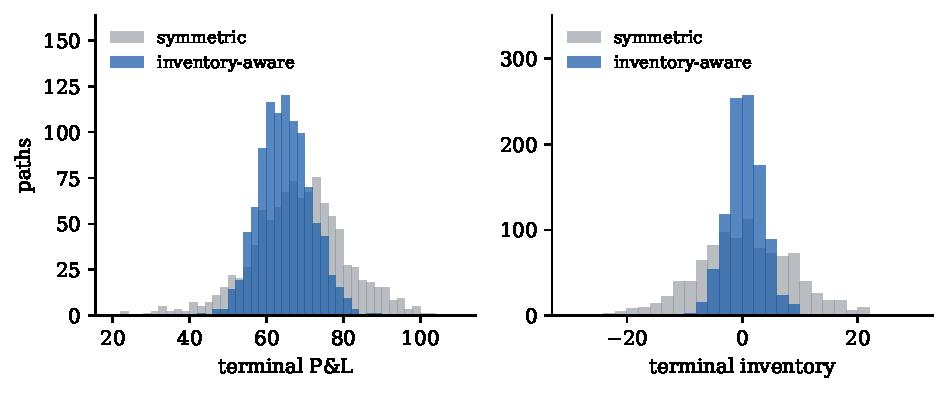
\includegraphics[width=\linewidth]{figures/fig5_mm.pdf}
\caption{Avellaneda--Stoikov market making ($\gamma=0.1$, 1000 simulated sessions). Skewing quotes against inventory keeps inventory near zero (right) and makes the P\&L distribution far tighter (left).}
\label{fig:mm}
\end{figure}

\section{How I built it}
\begin{itemize}[leftmargin=1.5em]
  \item \textbf{A known answer before any trust.} Every module was paired with a test against an exact result, an independent method (quadrature, Monte Carlo, finite differences) or a published table (Table~\ref{tab:valid}). Tests run on every change through GitHub Actions, on two Python versions.
  \item \textbf{Variance reduction and reproducibility.} Antithetic variates in every simulation, fixed random seeds, and checks that stochastic tests pass across several seeds, so that no test passes by luck.
  \item \textbf{Vectorised NumPy throughout.} The full test suite runs in about 11 seconds.
  \item \textbf{Honest defaults.} Costs are on by default; the IV solver returns NaN when a quote violates the arbitrage bounds; no size is suggested unless every hard gate passes.
\end{itemize}

\begin{table}[t]
\centering\small
\begin{tabular}{lll}
\toprule
Component & Check & Result\\
\midrule
Black--Scholes & put--call parity; textbook value & $1.4\times10^{-14}$; $10.4506$\\
Greeks (7) & central finite differences & $<10^{-6}$\\
Implied vol & round trip; arbitrage bounds & $2\times10^{-16}$; NaN outside bounds\\
American CRR & early-exercise premium; call $=$ European & $10.377 > 10.109$; within $5\times10^{-3}$\\
GARCH(1,1) & recover simulated $(\alpha,\beta)$ & within $(0.02, 0.03)$\\
SVI & recover a curve; detect arbitrage & RMSE $<10^{-5}$; flags spiky smile\\
Heston & BS limit; quadrature; Monte Carlo & $10^{-6}$; $10^{-8}$; within 4 s.e.\\
Heston calibration & noise-free / noisy surface & params to $10^{-4}$ / RMSE 0.16 vol pts\\
Delta hedging & locked-in P\&L; Derman--Kamal; drift & \$2.82; within a few \%; within 3 cents\\
Densities & BL vs lognormal; var swap at flat vol & $10^{-6}$; $10^{-4}$ relative\\
Event vol & desk worked example & 171\%, move 8.6\%\\
Kelly & analytic $f^*=1/6$ & 0.1655\\
Deflated Sharpe & false positives, best of 100 & naive $>90\%$, deflated $\le5\%$\\
Market making & Avellaneda--Stoikov (2008) table & spread 1.49; risk halved\\
\bottomrule
\end{tabular}
\caption{What each test checks. All 43 pass.}
\label{tab:valid}
\end{table}

\section{What I learned}
\begin{enumerate}[leftmargin=1.5em]
  \item \textbf{An option is a bet on volatility with a direction attached.} The hedging experiment made $\frac12\Gamma S^2(\sigma_r^2-\sigma_i^2)$ concrete: I can be right about direction and still lose to theta and IV crush.
  \item \textbf{Code that runs is not code that is right.} Most of my early errors were not in the formulas but in details. One example: a test of my Kelly optimiser kept failing until I realised that the grid itself limited its accuracy to 0.3\%.
  \item \textbf{The market prices a distribution, not a number.} The skew is information: it costs money in a variance swap and shows a fat left tail in the density.
  \item \textbf{The backtest is the most dangerous part.} Costs alone can turn a real pump into a loss, and searching over variants creates a Sharpe ratio from nothing. On synthetic data where I put the edge in myself, my strategy only broke even. That is the most important result in this paper, and it changes how I trade.
  \item \textbf{Physics habits transfer directly:} validating against exact solutions, checking convergence, and suspecting the numerics before the physics.
\end{enumerate}

\section{Limitations and next steps}
\begin{itemize}[leftmargin=1.5em]
  \item \textbf{The backtest uses synthetic data.} The next step is real historical option implied volatility, run with walk-forward splits and judged by the deflated Sharpe ratio.
  \item \textbf{The Monte Carlo exit IV is an at-the-money proxy,} not a full repricing of the surface.
  \item \textbf{Heston is calibrated to synthetic surfaces only.} Fitting it to a live chain, and comparing it with SVI, is the natural extension.
  \item \textbf{Smaller limits.} The scenario P\&L handles debit positions only, and the backtest uses one constant-maturity IV series.
\end{itemize}
This is research code for learning, not investment advice.

\begin{thebibliography}{99}\small
\bibitem{bs} F. Black and M. Scholes, ``The pricing of options and corporate liabilities,'' \emph{J. Political Economy} 81 (1973).
\bibitem{heston} S. Heston, ``A closed-form solution for options with stochastic volatility,'' \emph{Rev. Financial Studies} 6 (1993).
\bibitem{trap} H. Albrecher, P. Mayer, W. Schoutens and J. Tistaert, ``The little Heston trap,'' \emph{Wilmott Magazine} (2007).
\bibitem{lewis} A. Lewis, \emph{Option Valuation under Stochastic Volatility} (Finance Press, 2000).
\bibitem{gatheral} J. Gatheral, \emph{The Volatility Surface} (Wiley, 2006).
\bibitem{bl} D. Breeden and R. Litzenberger, ``Prices of state-contingent claims implicit in option prices,'' \emph{J. Business} 51 (1978).
\bibitem{cm} P. Carr and D. Madan, ``Towards a theory of volatility trading,'' in \emph{Volatility} (Risk Books, 1998).
\bibitem{dk} S. Kamal and E. Derman, ``When you cannot hedge continuously,'' \emph{Risk} (1999).
\bibitem{wilmott} P. Wilmott, \emph{Paul Wilmott Introduces Quantitative Finance}, 2nd ed. (Wiley, 2007).
\bibitem{psr} D. Bailey and M. López de Prado, ``The Sharpe ratio efficient frontier,'' \emph{J. Risk} 15 (2012); ``The deflated Sharpe ratio,'' \emph{J. Portfolio Management} 40 (2014).
\bibitem{as} M. Avellaneda and S. Stoikov, ``High-frequency trading in a limit order book,'' \emph{Quantitative Finance} 8 (2008).
\bibitem{garch} T. Bollerslev, ``Generalized autoregressive conditional heteroskedasticity,'' \emph{J. Econometrics} 31 (1986).
\end{thebibliography}

\end{document}
